\documentclass[a4paper,12pt]{ctexart}

\usepackage{listings}
\usepackage[colorlinks,linkcolor=black]{hyperref}
\usepackage{indentfirst}
\usepackage{xcolor}
\usepackage{graphicx}
\usepackage{geometry}
\geometry{top=2.5cm,bottom=3.0cm,left=2.0cm,right=2.0cm}
\lstset{
	columns=fixed,
	numbers=left,
	breaklines=true,
	frame=shadowbox,
	commentstyle=\color{gray},
	rulesepcolor= \color{gray},
	numberstyle= \small,
	keywordstyle= \color{red},
	stringstyle=\rmfamily\slshape\color[RGB]{128,0,0},
	showstringspaces=false, 
	morekeywords={my,asm},
	showtabs=false,
	tabsize=4,
	title=\lstname,
	basicstyle=\ttfamily
}


\title{Android中的MVP框架}
\author{A Fool}
\date{2019}

\begin{document}
	\maketitle
	\tableofcontents
	\section{MVP}
	\subsection{MVP概述}
	MVP 全称:Model-View-Presenter ;MVP 是从经典的模式MVC演变而来,它们的基本思想有相通的地方:Controller/Presenter负责逻辑的处理,Model提供数据,View负责显示。
	\begin{itemize}
		\item Model 定义用户界面所需要被显示的数据模型,一个模型包含着相关的业务逻辑。
		\item View 视图为呈现用户界面的终端,用以表现来自 Model 的数据,和用户命令路由再经过 Presenter 对事件处理后的数据。
		\item Presenter 包含着组件的事件处理,负责检索 Model 获取数据,和将获取的数据经过格式转换与 View 进行沟通。
	\end{itemize}
	\par MVP从MVC演变而来,通过表示器将视图与模型巧妙地分开。在该模式中,视图通常由表示器初始化,它呈现用户界面(UI)并接受用户所发出命令,但不对用户的输入作任何逻辑处理,而仅仅是将用户输入转发给表示器。通常每一个视图对应一个表示器,但是也可能一个拥有较复杂业务逻辑的视图会对应多个表示器,每个表示器完成该视图的一部分业务处理工作,降低了单个表示器的复杂程度,一个表示器也能被多个有着相同业务需求的视图复用,增加单个表示器的复用度。表示器包含大多数表示逻辑,用以处理视图,与模型交互以获取或更新数据等。模型描述了系统的处理逻辑,模型对于表示器和视图一无所知。
	\begin{figure}[!h]
		\centering
		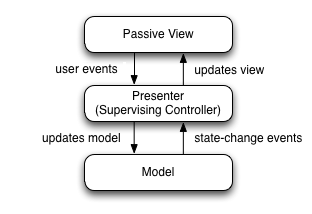
\includegraphics[]{image/1.png}
		\caption{MVP原理图}
	\end{figure}
	\begin{figure}[!h]
		\centering
		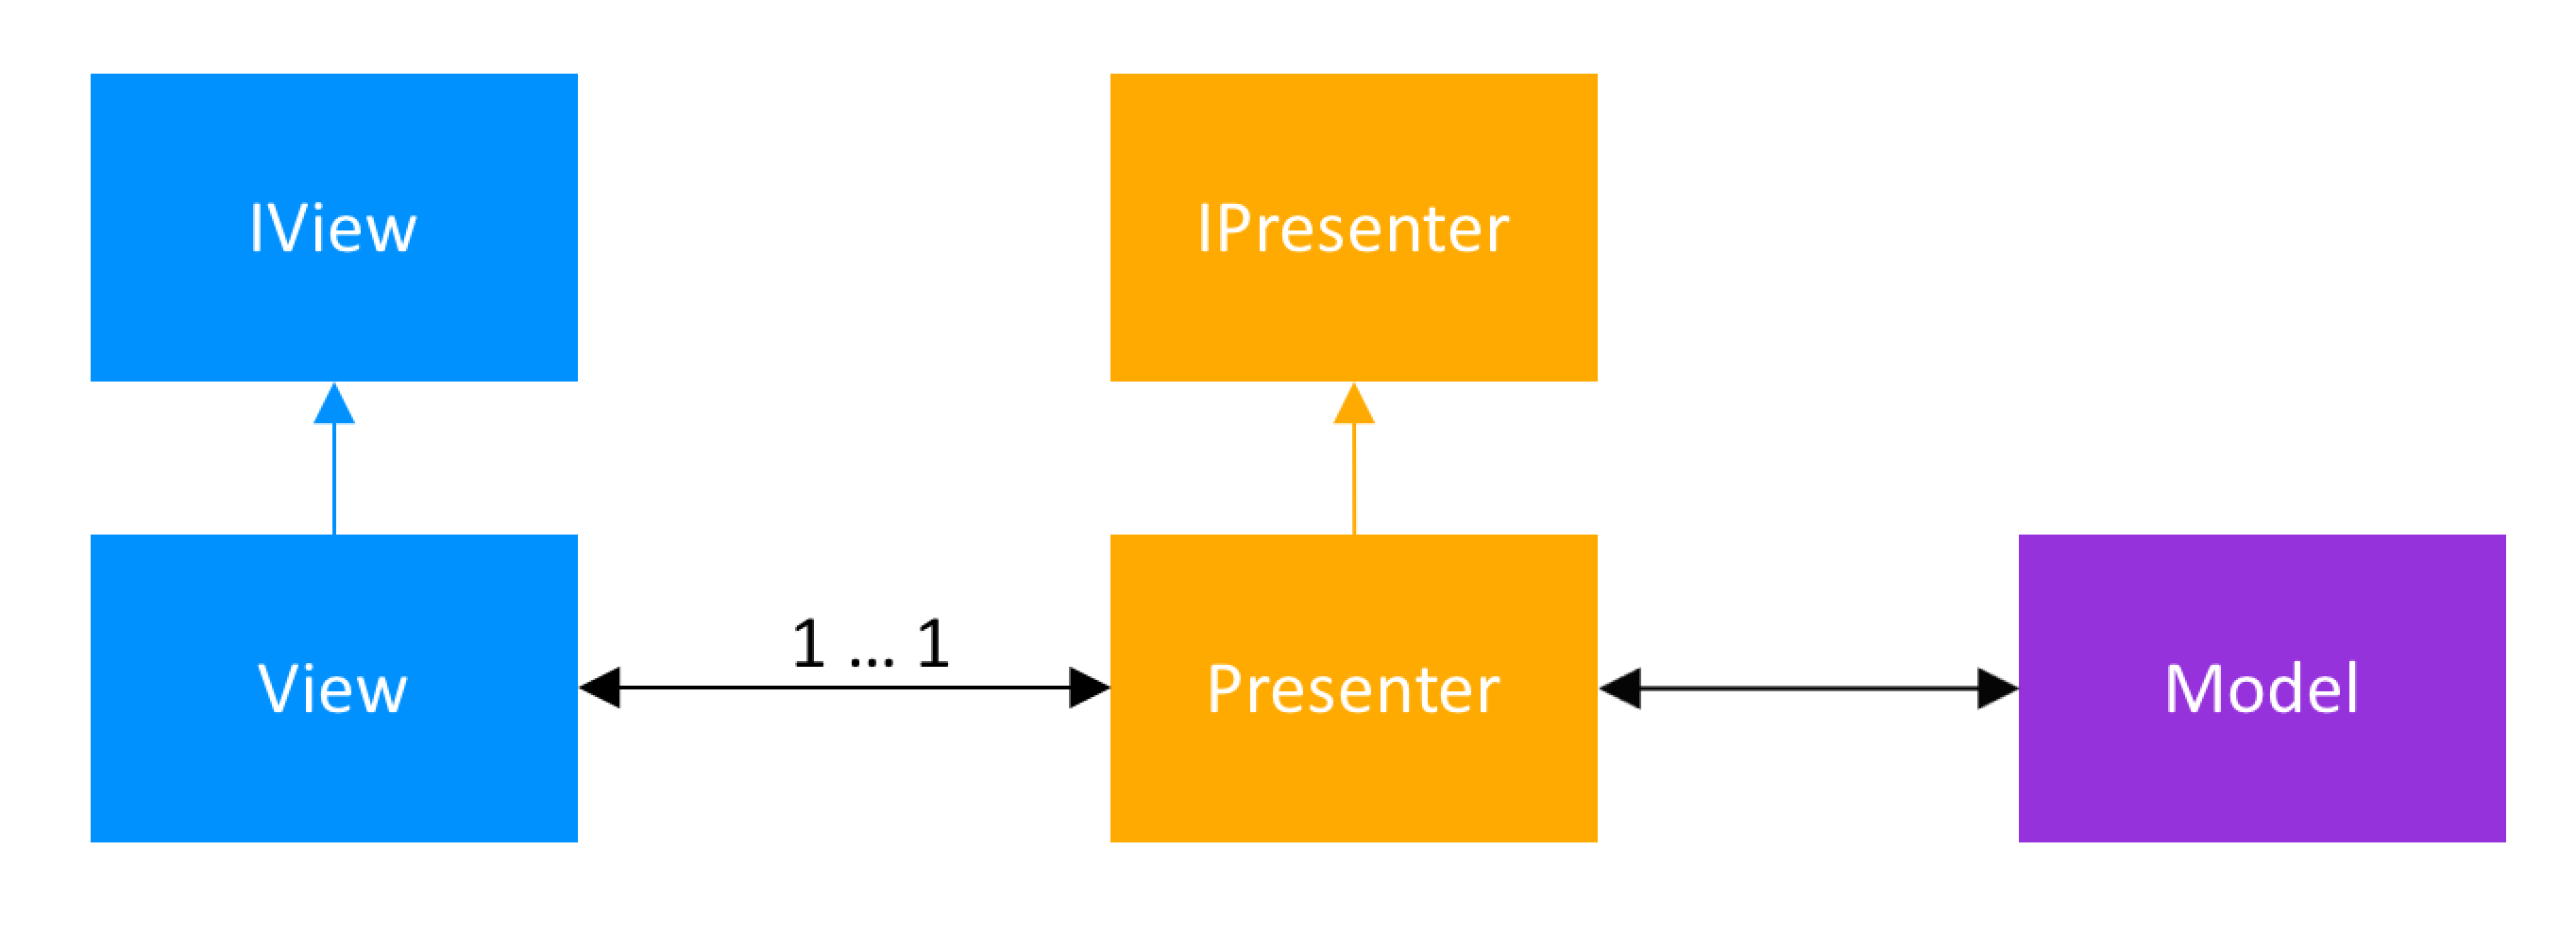
\includegraphics[width=0.8\textwidth]{image/2.png}
		\caption{Model-View-Presenter class structure}
	\end{figure}
	\subsection{优缺点}
	优点:
	\begin{enumerate}
		\item View与Model完全隔离,如果Model或View中的一方发生变化,只要交互接口不变,另一方就没必要对上述变化做出改变。这使得Model层的业务逻辑具有很好的灵活性和可重用性。
		\item Presenter与View的具体实现技术无关,采用诸如Windows表单、WPF、Web表单等用户界面构建技术中的任意一种来实现View层,都无需改变系统的其他部分。甚至为了使B/S,C/S部署架构能够被同时支持,应用程序可以用同一个Model层适配多种技术构建的View层。
		\item 可以进行View的模拟测试,在MVP模式中,View和Model之间没有直接依赖,开发者能够借助模拟对象注入测试两者中的任一方。
		\item 视图的变化总是比较频繁,将业务逻辑抽取出来,放在表示器中实现,使模块职责划分明显,层次清晰,一个表示器能复用于多个视图,而不需要更改表示器的逻辑,这增加了程序的复用性。
		\item 数据的处理由模型层完成,隐藏了数据,在数据显示时,表示器可以对数据进行访问控制,提高数据的安全性。
	\end{enumerate}
	\par 缺点:
	\par 增加了代码的复杂度,特别是针对小型Android应用的开发,会使程序冗余。
	\par 1. Presenter中除了应用逻辑以外,还有大量的View->Model,Model->View的手动同步逻辑,会导致Presenter臃肿,维护困难。
	\par 2. 视图的渲染过程也会放在Presenter中,造成视图与Presenter交互过于频繁,如果某特定视图的渲染很多,就会造成Presenter与该视图联系过于紧密,一旦该视图需要变更,那么Presenter也需要变更了,不能如预期的那样降低耦合度和增加复用性。
	\par 注:
	\begin{itemize}
		\item 如果要实现的UI比较复杂,而且相关的显示逻辑还跟Model有关系,就可以在View和Presenter之间放置一个Adapter。由这个Adapter来访问Model和View,避免两者之间的关联。而同时,因为Adapter实现了View的接口,从而可以保证与Presenter之间接口的不变。这样就可以保证View和Presenter之间接口的简洁,又不失去UI的灵活性。
		\item 在MVP模式里,View只应该有简单的Set/Get的方法,用户输入和设置界面显示的内容,除此就不应该有更多的内容,绝不容许直接访问Model--这就是与MVC很大的不同之处。
	\end{itemize}
	为什么MVP模式利于单元测试?
	\par Presenter将逻辑和UI分开了,里面没有Android代码,都是纯纯的java代码。我们可以直接对Presenter写Junit测试。
	\section{Android中的MVP}
\subsection{标准MVP模式}
\begin{itemize}
	\item BaseActivity: 提供Activity的抽象类;
	\item BasePresenter: Presenter的接口;
	\item BookBean: 实体Bean;
	\item BookCallBack: 返回CallBack接口,传递返回结果;
	\item BuyBookActivity: View层,负责数据显示;
	\item BuyBookAdapter: ListView适配器;
	\item BuyBookContract: 包含View和Presenter更接近本层功能的接口;
	\item BuyBookModel: Model层,负责网络请求;
	\item BuyBookPresenter: Presenter层,负责处理View和Model之间的交互。
\end{itemize}
\begin{lstlisting}[language=java]
//BaseActivity
public abstract class BaseActivity<T extends BasePresenter> extends Activity {
	protected T basepresenter;
	@Override
	protected void onCreate(@Nullable Bundle savedInstanceState) {
		super.onCreate(savedInstanceState);
		setContentView(getLayout());
		initView();
		basepresenter = initPresent();
		onPrepare();
	}
	abstract T initPresent();
	abstract int getLayout();
	abstract void initView();
	abstract void onPrepare();
}
\end{lstlisting}
\begin{lstlisting}[language=java]
//BasePresenter
public abstract class BasePresenter<T extends BaseActivity> {
	abstract void initData();
}
\end{lstlisting}
\begin{lstlisting}[language=java]
//BookBean
public class BookBean {
	private String name;
	private int number;
	private String time;
	//setter getter 构造器
}
\end{lstlisting}
\begin{lstlisting}[language=java]
//BookCallBack
public interface BookCallBack<T> {
	void onSuccess(T t);
	void onFail(String code);
}
\end{lstlisting}
\begin{lstlisting}[language=java]
//BuyBookActivity
public class BuyBookActivity extends BaseActivity<BuyBookPresenter> implements BuyBookContract.IBuyBookView {
	private ListView listView;
	private BuyBookAdapter adapter;
	@Override
	BuyBookPresenter initPresent() {
		return new BuyBookPresenter(this);
	}
	@Override
	int getLayout() {
		return R.layout.activity_buy;
	}
	@Override
	void initView() {
		listView = findViewById(R.id.list_view);
	}
	@Override
	void onPrepare() {
		adapter = new BuyBookAdapter(basepresenter.getAdapterData(), this);
		listView.setAdapter(adapter);
		basepresenter.initData();
	}
	@Override
	public void showToast(String msg) {
		Toast.makeText(this, msg, Toast.LENGTH_LONG).show();
	}
	@Override
	public void refreshAdapter() {
		adapter.notifyDataSetChanged();
	}
	@Override
	public void onEmpty() {
		listView.setEmptyView(null);
	}
}
\end{lstlisting}
\begin{lstlisting}[language=java]
//BuyBookAdapter
public class BuyBookAdapter extends BaseAdapter{
	private List<BookBean> list;
	private Context context;
	public BuyBookAdapter(List<BookBean> list, Context context) {
		this.list = list;
		this.context = context;
	}
	@Override
	public int getCount() {
		return list == null ? 0 : list.size();
	}
	@Override
	public Object getItem(int position) {
		return list == null ? null : list.get(position);
	}
	@Override
	public long getItemId(int position) {
		return position;
	}
	@Override
	public View getView(int position, View convertView, ViewGroup parent) {
		MyHolder myHolder = null;
		if (convertView == null) {
			convertView = View.inflate(context, R.layout.lst_item, null);
			myHolder = new MyHolder(convertView);
			convertView.setTag(myHolder);
		} else {
			myHolder = (MyHolder) convertView.getTag();
		}
		myHolder.name.setText(list.get(position).getName());
		myHolder.number.setText("(" + list.get(position).getNumber() + "人)");
		myHolder.time.setText(list.get(position).getTime());
		return convertView;
	}
	class MyHolder {
		TextView name;
		TextView number;
		TextView time;
		public MyHolder(View v) {
			name = v.findViewById(R.id.name);
			number = v.findViewById(R.id.number);
			time = v.findViewById(R.id.time);
		}
	}
}
\end{lstlisting}
\begin{lstlisting}[language=java]
//BuyBookContract
public class BuyBookContract {
	interface IBuyBookModel {
		void getTestData(BookCallBack<List<BookBean>> callBack);
		List<BookBean> getAdapterData();
	}
	
	interface IBuyBookPresenter {
		List<BookBean> getAdapterData();
	}
	interface IBuyBookView {
		void showToast(String msg);
		void refreshAdapter();
		void onEmpty();
	}
}
\end{lstlisting}
\begin{lstlisting}[language=java]
//BuyBookModel
public class BuyBookModel implements BuyBookContract.IBuyBookModel {
	private List<BookBean> list;
	public BuyBookModel() {
		this.list = new ArrayList<>();
	}
	@Override
	public void getTestData(final BookCallBack<List<BookBean>> callBack) {
		new Handler().postDelayed(new Runnable() {
			@Override
			public void run() {
				List<BookBean> tlist = new ArrayList<>();
				tlist.add(new BookBean("赵云", 1, "09-27 09:11"));
				tlist.add(new BookBean("赵云、隔壁老王、小王、典韦、貂蝉、林芳、曹操、刘备、关羽、黄忠、张飞、诸葛孔明", 10, "09-27 09:11"));
				tlist.add(new BookBean("黄忠、孙权、大乔", 50, "09-27 09:11"));
				tlist.add(new BookBean("大乔、小乔、貂蝉、孙尚香", 300, "09-27 09:11"));
				Random rd = new Random();
				int N = rd.nextInt(10);
				if (N > 5) {
					callBack.onSuccess(tlist);
				} else {
					callBack.onFail("请求失败");
				}
			}
		}, 1000);
	}
	
	@Override
	public List<BookBean> getAdapterData() {
		return list;
	}
}
\end{lstlisting}
\begin{lstlisting}[language=java]
//BuyBookPresenter
public class BuyBookPresenter extends BasePresenter<BuyBookActivity> implements BuyBookContract.IBuyBookPresenter {
	private BuyBookContract.IBuyBookView view;
	private BuyBookModel model;
	public BuyBookPresenter(BuyBookContract.IBuyBookView view) {
		this.view = view;
		this.model = new BuyBookModel();
	}
	@Override
	void initData() {
		model.getTestData(new BookCallBack<List<BookBean>>() {
			@Override
			public void onSuccess(List<BookBean> bookBeans) {
				model.getAdapterData().addAll(bookBeans);
				view.refreshAdapter();
			}
			@Override
			public void onFail(String code) {
				view.showToast(code);
				view.onEmpty();
			}
		});
	}
	@Override
	public List<BookBean> getAdapterData() {
		return model.getAdapterData();
	}
}
\end{lstlisting}

\subsection{MVP常用实例二}
\begin{itemize}
	\item MainActivity:View层,专注视图处理;
	\item MVPCallback:用于返回结果;
	\item MVPContract:封装View、Presenter接口;
	\item MVPModel:Mode层,网络交互;
	\item MVPPresenter:Presenter层,处理View请求,与Model交互。
\end{itemize}
\begin{lstlisting}[language=java]
//MainActivity
public class MainActivity extends AppCompatActivity implements MVPContract.IMVPView {

	private ProgressDialog progressDialog;
	private MVPContract.IMVPPresenter presenter;
	
	@Override
	protected void onCreate(Bundle savedInstanceState) {
		super.onCreate(savedInstanceState);
		setContentView(R.layout.activity_main);
		
		initView();
		setPresenter();
	}
	protected void initView() {
		progressDialog = new ProgressDialog(this);
		progressDialog.setCancelable(false);
		progressDialog.setMessage("正在加载");
	}
	
	@Override
	public void setPresenter() {
		presenter = new MVPPresenter(this);
	}
	
	@Override
	public void showLoading() {
		if (!progressDialog.isShowing()) {
			progressDialog.show();
		}
	}
	
	@Override
	public void hideLoading() {
		if (progressDialog.isShowing()) {
			progressDialog.dismiss();
		}
	}
	
	@Override
	public void showData(String data) {
		Toast.makeText(this, data, Toast.LENGTH_SHORT).show();
	}
	
	@Override
	public void showFailureMessage(String msg) {
		Toast.makeText(this, msg, Toast.LENGTH_SHORT).show();
	}
	
	@Override
	public void showErrorMessage() {
		Toast.makeText(this, "网络请求数据出现异常", Toast.LENGTH_SHORT).show();
	}
	
	public void getData(View view){
		presenter.getData("normal");
	}
	
	public void getDataForFailure(View view){
		presenter.getData("failure");
	}
	
	public void getDataForError(View view){
		presenter.getData("error");
	}
}
\end{lstlisting}
\begin{lstlisting}[language=java]
//MVPCallback
public interface MVPCallback {
	void onSuccess(String data);
	void onFailure(String msg);
	void onError();
	void onComplete();
}
\end{lstlisting}
\begin{lstlisting}[language=java]
//MVPContract
public class MVPContract {
	interface IMVPView {
		void setPresenter();
		void showLoading();
		void hideLoading();
		void showData(String data);
		void showFailureMessage(String msg);
		void showErrorMessage();
	}
	interface IMVPPresenter {
		void start();
		void getData(String params);
	}
}
\end{lstlisting}
\begin{lstlisting}[language=java]
//MVPModel
public class MVPModel {
	public void getNetData(final String param, final MVPCallback callback) {
		new Handler().postDelayed(new Runnable() {
			@Override
			public void run() {
				switch (param) {
				case "normal":
				callback.onSuccess("请求成功");
				break;
				case "failure":
				callback.onFailure("请求失败");
				break;
				case "error":
				callback.onError();
				break;
			}
			callback.onComplete();
			}
		}, 2000);
	}
}
\end{lstlisting}
\begin{lstlisting}[language=java]
//MVPPresenter
public class MVPPresenter implements MVPContract.IMVPPresenter{
	private MVPContract.IMVPView view;
	private MVPModel model;
	
	public MVPPresenter(MVPContract.IMVPView view) {
		this.view = view;
		model = new MVPModel();
	}
	
	@Override
	public void start() {
	}
	
	public void getData(String params) {
		view.showLoading();
		model.getNetData(params, new MVPCallback() {
			@Override
			public void onSuccess(String data) {
				view.showData(data);
			}
			
			@Override
			public void onFailure(String msg) {
				view.showFailureMessage(msg);
			}
			
			@Override
			public void onError() {
				view.showErrorMessage();
			}
			
			@Override
			public void onComplete() {
				view.hideLoading();
			}
		});
	}
}
\end{lstlisting}
\subsection{MVP常用实例改造}
实体Bean:
\begin{lstlisting}[language=java]
//请求返回解析Gson辅助类
public class ResponseBean {
	private WeatherBean weatherinfo;
	public ResponseBean(WeatherBean weatherBean) {
		this.weatherinfo = weatherBean;
	}
	public WeatherBean getWeatherBean() {
		return weatherinfo;
	}
	public void setWeatherBean(WeatherBean weatherBean) {
		this.weatherinfo = weatherBean;
	}
}
//真正实体Bean
public class WeatherBean {
	private String city;
	private String cityid;
	private String temp1;
	private String temp2;
	private String weather;
	private String img1;
	private String img2;
	private String ptime;
	// setter getter 构造器...
}
\end{lstlisting}
\subsubsection{普通实例一}
通过简单地OkHttp获取网络数据,Gson解析后通过Handler显示到View,这里一气呵成,将Controller和View混淆在一起,
随着功能的增加,Activity的体量会迅速上升。
\begin{lstlisting}[language=java]
public class MainActivity extends AppCompatActivity {
	private TextView textView;
	String temp;
	private Handler handler = new Handler(){
		@Override
		public void handleMessage(Message msg) {
			switch (msg.what) {
				case 1:
					textView.setText(temp);
					break;
			}
		}
	};
	
	@Override
	protected void onCreate(Bundle savedInstanceState) {
		super.onCreate(savedInstanceState);
		setContentView(R.layout.activity_main);
		textView = findViewById(R.id.text_weather);
		getTextInfo();
	}
	protected void getTextInfo(){
		OkHttpClient client = new OkHttpClient();
		Request request = new Request.Builder()
			.url("http://www.weather.com.cn/data/cityinfo/101010100.html")
			.build();
		Call call = client.newCall(request);
		call.enqueue(new Callback() {
		@Override
		public void onFailure(Call call, IOException e) {
			textView.setText("失败");
		}
		
		@Override
		public void onResponse(Call call, Response response) throws IOException {
			Gson gson = new Gson();
			String t = response.body().string();
			ResponseBean responseBean = gson.fromJson(t,ResponseBean.class);
			WeatherBean weatherBean = responseBean.getWeatherBean();
			temp = weatherBean.getCity() + " " + weatherBean.getTemp1() + " " + weatherBean.getTemp2() + " " + weatherBean.getWeather();
			Message msg = new Message();
			msg.what = 1;
			handler.sendMessage(msg);
		}
		});
	}
}
\end{lstlisting}
\subsubsection{简单MVP实现}
\begin{enumerate}
	\item 先定义一个接口RequestView1,用来针对View需要做出的动作;
	\item 让Activity实现RequestView1,构成View层;
	\item 再创建一个类,封装网络请求过程,与Bean构成Model层;
	\item 再创建一个类,处理Model层和View层交互,构成Presenter层。
\end{enumerate}
\begin{lstlisting}[language=java]
public interface RequestView1 {
	//请求时展示加载
	void requestLoading();
	//请求成功
	void resultSuccess(WeatherBean result);
	//请求失败
	void resultFailure(String result);
}
\end{lstlisting}
\begin{lstlisting}[language=java]
public class MainActivity extends AppCompatActivity implements RequestView1 {
	
	@FieldView(R.id.tv_text)
	private TextView textView;
	private RequestPresenter1 presenter;
	
	@Override
	protected void onCreate(Bundle savedInstanceState) {
		super.onCreate(savedInstanceState);
		setContentView(R.layout.activity_main);
		ViewFind.bind(this);
		
		//创建Presenter
		presenter = new RequestPresenter1(this);
	}
	
	//点击事件
	public void request(View view) {
		presenter.clickRequest("101010100");
	}
	
	//请求时加载
	@Override
	public void requestLoading() {
		textView.setText("请求中,请稍后...");
	}
	
	//请求成功
	@Override
	public void resultSuccess(WeatherBean result) {
		//成功
		textView.setText(result.getWeatherinfo().toString());
	}
	
	//请求失败
	@Override
	public void resultFailure(String result) {
		//失败
		textView.setText(result);
	}
}
\end{lstlisting}
\begin{lstlisting}[language=java]
public class RequestMode1 {

	private static final String BASE_URL = "http://www.weather.com.cn/";
	
	public void request(String detailId, Callback<WeatherBean> callback){
		//请求接口
		Retrofit retrofit  = new Retrofit.Builder()
		//代表root地址
		.baseUrl(BASE_URL)
		.addConverterFactory(ScalarsConverterFactory.create())
		.addConverterFactory(GsonConverterFactory.create())
		.build();
		
		ApiService apiService = retrofit.create(ApiService.class);
		
		//请求
		Call<WeatherBean> weatherBeanCall = apiService.requestWeather(detailId);
		
		weatherBeanCall.enqueue(callback);
	}
}
\end{lstlisting}
\begin{lstlisting}[language=java]
//需要View和Model层的引用
public class RequestPresenter1 {
	
	private final RequestView1 mRequestView;
	private final RequestMode1 mRequestMode;
	
	public RequestPresenter1(RequestView1 requestView) {
		this.mRequestView = requestView;
		this.mRequestMode = new RequestMode1();
	}
	
	public void clickRequest(final String cityId){
		//请求时显示加载
		mRequestView.requestLoading();
		
		//模拟耗时,可以展示出loading
		new Handler().postDelayed(new Runnable() {
			@Override
			public void run() {
				mRequestMode.request(cityId, new Callback<WeatherBean>() {
				@Override
				public void onResponse(Call<WeatherBean> call, Response<WeatherBean> response) {
					mRequestView.resultSuccess(response.body());
				}
				
				@Override
				public void onFailure(Call<WeatherBean> call, Throwable t) {
					mRequestView.resultFailure(Log.getStackTraceString(t));
				}
				});
			}
		},1000);
	}
}
\end{lstlisting}
\subsubsection{改进-解决内存泄露}
\noindent 因为如果在网络请求的过程中Activity就关闭了,Presenter还持有了V层的引用,也就是MainActivity,就会内存泄露。
\\ 解决办法:将P层和V层的关联抽出两个方法,一个绑定,一个解绑,在需要的时候进行绑定V层,不需要的时候进行解绑就可以了。
只需要修改上面Presenter中的构造代码,不需要在构造中传递V层了,然后再写一个绑定和解绑的方法,最后修改Activity创建Presenter时进行绑定,在onDestroy中进行解绑。
\begin{lstlisting}[language=java]
//Presenter层
public class RequestPresenter2 {
	
	private RequestView2 mView;
	private RequestMode2 mMode;
	
	public RequestPresenter2() {
		mMode = new RequestMode2();
	}
	public void clickRequest(final String cityId) {
		//...
	}
	//绑定
	public void attach( RequestView2 view) {
		this.mView = view;
	}
	//解绑
	public void detach() {
		mView = null;
	}
	//取消网络请求
	public void interruptHttp(){
		mMode.interruptHttp();
	}
}
\end{lstlisting}
\begin{lstlisting}[language=java]
//1. 是会内存泄露,因为persenter一直持有Activity,如果一个发了一个请求,但是网络有点慢,这个时候退出Activity,那么请求回来后还是会调用Activity的回调方法,这里还是因为一直持有的问题。
//2. 如果已经退出了当前界面,这个请求也没有用了,这个时候我们可以断开请求
/解决:
//1. 增加绑定和解绑的方法来解决内存泄露和退出后还会回调的问题;
//2. 增加断开网络连接的方法。
public class MainActivity extends AppCompatActivity implements RequestView2 {
	//...
	protected void onCreate(Bundle savedInstanceState) {
		//...
		presenter = new RequestPresenter2();
		presenter.attach(this);
	}
	//...
	protected void onDestroy() {
		super.onDestroy();
		presenter.detach();
		presenter.interruptHttp();
	}
}
\end{lstlisting}
\par 仍存在问题:应用中肯定不可能只有一个模块,每个模块都对应着一个V层和P层,那这样的话每个Presenter中都要定义绑定和解绑的方法,而Activity中对应的也要调用这绑定和解绑的两个方法,代码冗余。
\subsubsection{再次改进-简单抽象}
\begin{enumerate}
	\item 创建一个基类View,让所有View接口都必须实现,这个View可以什么都不做只是用来约束类型的;
	\item 创建一个基类的Presenter,在类上规定View泛型,然后定义绑定和解绑的抽象方法,让子类去实现,对外在提供一个获取View的方法,,让子类直接通过方法获取View。
	\item 创建一个基类的Activity,声明一个创建Presenter的抽象方法,因为要帮子类去绑定和解绑那么就需要拿到子类的Presenter才行,但是又不能随便一个类都能绑定的,因为只有基类的Presenter中才定义了绑定和解绑的方法,所以同样的在类上可以声明泛型在,方法上使用泛型来达到目的。
	\item 修改Presenter和Activity中的代码,各自继承自己的基类并去除重复代码。
\end{enumerate}
\begin{lstlisting}[language=java]
public interface IMvpBaseView4 {
}
\end{lstlisting}
\begin{lstlisting}[language=java]
public abstract class AbstractMvpPersenter4<V extends IMvpBaseView4> {
	private V mMvpView;
	
	public void attachMvpView(V view){
		this.mMvpView = view;
	}
	
	public void detachMvpView(){
		mMvpView = null;
	}
	
	public V getmMvpView() {
		return mMvpView;
	}
}
\end{lstlisting}
\begin{lstlisting}[language=java]
public abstract class AbstractMvpActivity<V extends IMvpBaseView4, P extends AbstractMvpPersenter4<V>> extends AppCompatActivity implements IMvpBaseView4 {
	private P presenter;
	@Override
	protected void onCreate(@Nullable Bundle savedInstanceState) {
		super.onCreate(savedInstanceState);
		
		//创建Presenter
		if (presenter == null) {
			presenter = createPresenter();
		}
	
		if (presenter == null) {
			throw new NullPointerException("presenter 不能为空!");
		}
		//绑定view
		presenter.attachMvpView((V) this);
	}
	
	@Override
	protected void onDestroy() {
		super.onDestroy();
		//解除绑定
		if (presenter != null) {
			presenter.detachMvpView();
		}
	}
	
	/**
	* 创建Presenter
	* @return 子类自己需要的Presenter
	*/
	protected abstract P createPresenter();
	
	/**
	* 获取Presenter
	* @return 返回子类创建的Presenter
	*/
	public P getPresenter() {
		return presenter;
	}
}
\end{lstlisting}
\begin{lstlisting}[language=java]
public class RequestPresenter4 extends AbstractMvpPersenter4<RequestView4> {

	private final RequestMode4 mRequestMode;
	
	public RequestPresenter4() {
		this.mRequestMode = new RequestMode4();
	}
	
	public void clickRequest(final String cityId){
	//...
	}
	public void interruptHttp(){
		mRequestMode.interruptHttp();
	}
}
\end{lstlisting}
\begin{lstlisting}[language=java]
public interface RequestView4  extends IMvpBaseView4{
	void requestLoading();
	void resultSuccess(WeatherBean result);
	void resultFailure(String result);
}

public class MainActivity extends AbstractMvpActivity<RequestView4, RequestPresenter4> implements RequestView4 {
	private RequestPresenter4 presenter;
	//...
	//这里在父类AbstractMvpActivity构造函数中实现绑定
	protected RequestPresenter4 createPresenter() {
		return new RequestPresenter4();
	}
	//...
}
\end{lstlisting}
\subsubsection{高级抽象-使用注解、工厂模式、代理模式、策略模式}
\url{http://www.androidchina.net/7961.html}
\end{document}